% -*- TeX:de -*-
\NeedsTeXFormat{LaTeX2e}
\documentclass[12pt,a4paper]{article}
\usepackage[german]{babel} % german text
\usepackage[DIV12]{typearea} % size of printable area
\usepackage[T1]{fontenc} % font encoding
%\usepackage[latin1]{inputenc} % most likely on Windows
\usepackage[utf8]{inputenc} % probably on Linux
\usepackage{multicol}

% PLOTTING
\usepackage{pgfplots} 
\usepackage{pgfplotstable}
\usepackage{url}
\usepackage{graphicx} % to include images
\usepackage{tikz}
\usepackage{subfigure} % for creating subfigures
\usepackage{amsmath} % a bunch of symbols
\usepackage{amssymb} % even more symbols
\usepackage{booktabs} % pretty tables
\usepackage{makecell} % multi row table heading

% a floating environment for circuits
\usepackage{float}
\usepackage{caption}

%\newfloat{circuit}{tbph}{circuits}
%\floatname{circuit}{Schaltplan}

% a floating environment for diagrams
%\newfloat{diagram}{tbph}{diagrams}
%\floatname{diagram}{Diagramm}
\pgfplotsset{compat=1.8}
\selectlanguage{german} % use german

\begin{document}

%%%%%%% DECKBLATT %%%%%%%
\thispagestyle{empty}
			\begin{center}
			\Large{Fakultät für Physik}\\
			\end{center}
\begin{verbatim}


\end{verbatim}
							%Eintrag des Wintersemesters
			\begin{center}
			\textbf{\LARGE SS 14}
			\end{center}
\begin{verbatim}


\end{verbatim}
			\begin{center}
			\textbf{\LARGE{Physikalisches Praktikum\\ für das Bachelorstudium}}
			\end{center}
\begin{verbatim}




\end{verbatim}

			\begin{center}
			\textbf{\LARGE{PROTOKOLL}}
			\end{center}
			
\begin{verbatim}

\end{verbatim}

			\begin{flushleft}
			\textbf{\Large{Experiment (Nr., Titel): PS2 - Schwingungen 2}\\
							%Experiment Nr. und Titel statt den Punkten eintragen
			\LARGE{PS2}}	
			\end{flushleft}

\begin{verbatim}

\end{verbatim}	
							%Eintragen des Abgabedatums, oder des Erstelldatums des Protokolls
			\begin{flushleft}
			\textbf{\Large{Datum:}} \Large{12.06.2014}
			\end{flushleft}
			
\begin{verbatim}
\end{verbatim}
							%Namen der Protokollschreiber
		\begin{flushleft}
			\textbf{\Large{Namen:}} \Large{Patrick Braun, Johannes Kurz}
			\end{flushleft}

\begin{verbatim}


\end{verbatim}
							%Kurstag und Gruppennummer, zb. Fr/5
			\begin{flushleft}
			\textbf{\Large{Kurstag/Gruppe:}} \Large{DO/4}
			\end{flushleft}

\begin{verbatim}

\end{verbatim}
							%Name des Betreuers, das Praktikum betreute.
			\begin{flushleft}
			\LARGE{\textbf{Betreuer:}}	\Large{Wilhelm Markowitsch}	
			\end{flushleft}

%%%%%%% DECKBLATT ENDE %%%%%%%
\pagebreak
\setlength{\columnsep}{20pt}
\begin{multicols}{2}

%%%%%%%%%%%%%%%%%%%%%%%%%%%%%%%%%%%%%%%%%%%%%%%%

%\begin{figure}[H]
%	\centering
%	\includegraphics[scale=0.35]{./figure/beugung.png}
%	\caption{Beugungsmuster Einzelspalt (echtes Foto; schwarz durch weiß ersetzt)}
%	\label{fig:beugungsmuster}
%\end{figure}


%\begin{figure}[H]
%	\centering
%	\pgfplotstabletypeset[
%			columns={abstand, n},
%			col sep=&,
%			columns/abstand/.style={precision=2, zerofill, column name=\makecell{$Abstand$\\$(\pm 0.05)[mm]$} }, 
%			columns/n/.style={column name=\makecell{$n$\\$(Ordnung)$}, precision=0},
%			every head row/.style={before row=\hline,after row=\hline\hline},
%			every last row/.style={after row=\hline},
%			every first column/.style={column type/.add={|}{} },
%			every last column/.style={column type/.add={}{|} }
%			]{
%			abstand & n
%			12.9 & 1
%			24.45 & 2
%			37.40 & 3
%			49.35& 4
%			62.45 & 5
%			74.45 & 6
%			87.45 & 7
%			100.25 & 8
%			
%			}
%	\caption{Messwerte Einzelspalt}
%	\label{tab:werte_einzelspalt}
%\end{figure}


%%%%%%%%%%%%%%%%%%%%%%%%%%%%%%%%%%%%%%%%%%%%%%%%
%%%%%%%%%%%%%%%%%%%%%%%%%%%%%%%%%%%%%%%%%%%%%%%%


%\section{Schwingungen 2}
\noindent In PS2 geht es, ähnlich wie in PS1, um die Darstellung und Erforschung von Schwingungen, Dämpfungen, Kopplungen und getriebene Schwingungen.\\
Während in Schwingungen I jedoch mechanische Oszillatoren (Pendel und Lautsprecher) betrachtet werden, geht es in PS2 um einen elektrischen Oszillator, einen Schwingkreis.

%%%%%%%%%%%%%%%%%%%%%%%%%%%%%%%%%%%%%%%%%%%%%%%%%%%%%%%%%%%%%%%%%%%%%%%
\section{Grundlagen:}


%TODO: Schaltbild Schwingkreis
Ein Schwingkreis ist eine geschlossene Schaltung aus einem Kondensator und einer Spule in Serie. Weiters kann ein (ohmscher) Dämpfungswiderstand Teil der Schaltung sein, zumindest ist der Schwingkreis jedoch durch den Leitungswiderstand niemals völlig ungedämpft (wie ja auch ein mechanisches Pendel).\\

\subsection{Schwingkreis mit Dämpfung}
\noindent Ist der Kondensator (Kapazität $C$) geladen und der Kreis wird geschlossen, beginnt er sich zu entladen. Damit baut sich ein Strom in der Schaltung auf.\\
Die Änderung des Stromes erzeugt, nach dem Induktionsgesetz, ein Magnetfeld in der Spule (Induktivität $L$), und dadurch eine Spannung $U_L$, die der Kondensatorspannung entgegengesetzt ist (Abb.\ref{fig:schwingkreis_skizze}).\\
Zusammen ergibt sich
$$L\cdot \frac{dI}{dt} + R\cdot I - \frac{q}{C} = 0$$
und mit:\\
\indent $I = -\frac{dq}{dt}$\\
\indent $\delta = \frac{R}{2\cdot L}$\\
\indent $\omega_0=\sqrt{\frac{1}{L\cdot C}}$\\
die Schwingungsgleichung:
$$\frac{d^2q}{dt^2} + 2\delta\cdot \frac{dq}{dt} + \omega_0^2\cdot q = 0$$


\begin{figure}[H]
	\centering
	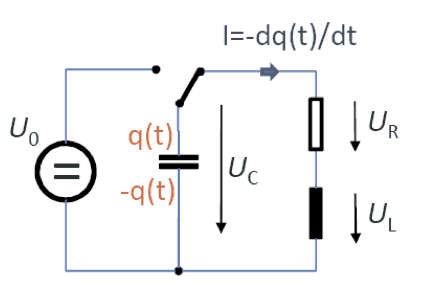
\includegraphics[scale=1.1]{./figure/schwingkreis_skizze.png}
	\caption{geschlossener Schwingkreis}
	\label{fig:schwingkreis_skizze}
\end{figure}



\noindent Diese ist völlig analog zur mechanischen Schwingungsgleichung (siehe PS1) mit einer Lösung:
$$q(t) = q_0 \cdot e^{-\delta t}\cdot cos(\omega_{0d}t  + \phi)$$
\noindent bei Anfangsbedingungen $I(0) = 0$ und $q(0) = q_0$.\\
$\delta$... Dämpfungsterm\\
$\omega_{0d}$...Eigenkreisfrequenz der gedämpften Schwingung\\

\noindent Ebenso analog zum mechanischen Oszillator gilt für die (theoretische) Eigenfrequenz des völlig ungedämpften Systems:
$$\omega_0 = \sqrt{\omega_{0d}^2 + \delta^2}$$
\noindent Die Dämpfung bewirkt also ein exponentielles Abklingen der Amplitude:
$$A(t) = A_0 \cdot e^{-\delta t}$$
$$ln(\frac{A_i}{A_0}) = -\delta t_i$$
Der Gütefaktor Q ist definiert als
$$Q = \frac{\omega_{0d}}{2\delta}$$

\subsection{Erzwungene Schwingung}
Der Schwingkreis kann, ebenso wie der mechanische Oszillator, durch periodisches Zuführen von Energie getrieben werden. Diese wird ausgedrückt durch eine periodische Funktion, rechts vom $=$.
$$\frac{d^2U_C}{dt^2} + 2 \delta\frac{dU_C}{dt} + \omega_{0}^2U_C = \frac{U_0}{LC} cos(\omega t)$$

Das System schwingt mit der antreibende Frequenz $\omega$ von der auch die Amplitude abhängt. Liegt $\omega$ nahe bei $$\omega_{max} = \sqrt{\omega_0^2 - 2\delta^2}$$gibt es, wie im mechanischen Fall, Resonanz.\\
Die Amplitude der getrieben Schwingung ist dabei gegeben durch
$$U_{C0} = U_0 \cdot \frac{\omega_0^2}{\sqrt{ (\omega_0^2 - \omega^2) + 4\delta^2 \omega^2}}$$

\noindent Aufgetragen gegen $\omega$ ergibt sich die Resonanzkurve des Oszillators mit dem Resonanzpeak bei $\omega_{max}$.\\
Die Stärke der Resonanz, also die Amplitude im Resonanzfall, ist nur durch die Dämpfung beschränkt. (Bei sehr kleinem $\delta$ bzw großem Q kann es daher zur Resonanzkatastrophe kommen, in diesem Fall eine Spannungsspitze.)\\

\noindent Außerdem wird noch die Phasenverschiebung $\phi$ zwischen der treibenden Spannung und der Kondensatorspannung betrachtet:
$$tan(\phi) = \frac{2 \delta \omega}{\omega^2 - \omega_0^2}$$

\subsection{Gekoppelte Schwingkreise}
%TODO Schaltplan Kopplung

In PS1 wurde eine gekoppelte Schwingung zweier Pendel betrachtet, die über einen Faden, an dem eine Kopplungmasse montiert ist, verbunden waren.\\
Aus der Lösung der Bewegungsgleichung kommen im mechanischen Fall die 2 Eigenfrequenzen für die gleichsinnige bzw. die gegensinnige Schwingung. Aus diesen lässt sich ein Kopplungsfaktor $K$ berechnen. Außerdem wurde im Schwebungsfall die Frequenz des Schwebungsamplituden-Verlaufs $\omega_S$ sowie der Pendelfrequenz während der Schwebung $\omega_m$ gemessen.
$$K=\frac{\omega_{geg}^2-\omega_{gl}^2}{\omega_{geg}^2+\omega_{gl}^2}=
\frac{2\omega_S \omega_m}{\omega_{S}^2+\omega_{m}^2}=\frac{C}{C_K + C}$$

\noindent Für den Schwingkreis lassen sich $\omega_{gegen}$ und $\omega_{gleich}$ nicht einfach durch manuelles Auslenken herstellen und messen, die Zusammenhänge sind jedoch ähnlich.\\
Die Kopplung kann über Strom oder Spannung erzeugt werden; hier bewirkt ein zusätzlicher, zwischen die beiden Schwingkreise geschalteter Kondensator, eine Spannungskopplung (Abb.\ref{fig:kopplung_skizze}).

\begin{figure}[H]
	\centering
	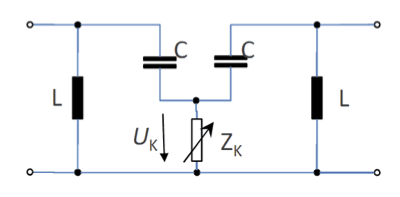
\includegraphics[scale=1.1]{./figure/kopplung_skizze.png}
	\caption{Schaltbild zweier gekoppelter Schwingkreise geschlossener Schwingkreis}
	\label{fig:kopplung_skizze}
\end{figure}






\pagebreak
\section{Versuchsaufbau:}

Alle Versuche in PS2 werden auf einem Steckbrett und mit, in entsprechenden Gehäusen verbauten, Bauteilen aufgebaut. Zur Messung der Amplituden und Schwingungsperioden dient ein \emph{Digitaloszilloskop TDS2000B}.\\
Sowohl die Kondensator-Spannung im ersten Teil, als auch die anregende Signalspannung in den beiden anderen Versuchen werden von einem \emph{Hameg HM 80-30} - Funktionsgenerator erzeugt. 

\subsection{Schwingkreis mit Dämpfung}

Die Schaltung wird wie in Abb.\ref{fig:schwingkreis_aufbau} aufgebaut:\\
Rechts befindet sich die Schleife mit dem Schwingkreis selbst. Channel 2 am Oszilloskop misst den Spannungsverlauf am Schwingkreiskondensator. Channel 1 misst den Spannungsverlauf des Signalgenerators. C' ist ein Einkoppelkondensator, der nicht nur für die erzwungene Schwingung benötigt wird, sondern auch hier den gewünschten Pattern der Versorgungsspannung erzeugt:\\
Der Signalgenerator erzeugt eine Rechteckswelle (20kHz). Jeder Spannungssprung entpricht einem kurzen, extrem hochfrequenten Signal, das dazu führt, dass C' für kurze Zeit durchlässig wird und so einen kurzen Spannungsimpuls in den Schwingkreis lässt. Dieser regt den Schwingkreis an, der wiederum, seiner Dämpfung entsprechend, ausschwingt bis zum nächsten Impuls.\\
Vom Signalgenerator wird ein Triggersignal direkt ans Oszilloskop gesendet, um eine präzise Darstellung des periodischen Vorgangs zu ermöglichen.\\

\noindent Mit dem Cursor des Oszilloskops werden mehrere Perioden und ihre Amplituden vermessen, zuerst ohne zusätzliche Dämpfung, danach mit einem Widerstand $R_D=2.2\Omega \pm 10\%$.\\
Aus einem linearen Fit aus den Logarithmen mehrerer Amplituden gegen die Zeit aufgetragen, lässt sich der Dämpfungskoeffizient $\delta$, und gemeinsam mit der Frequenz $\omega_{0d}$ die Eigenfrequenz $\omega_0$ sowie der Gütefaktor Q des Oszillators bestimmen.\\
Außerdem kann die Kapazität des Schwingkreiskondensators sowie der Eigenwiderstand der Spule berechnet werden.\\

\noindent Zuletzt wird mittels eines Potentiometers als variabler Widerstand, der Widerstand, an dem der aperiodische Grenzfall auftritt ($\delta = \omega_0$), gesucht.


\subsection{Erzwungene Schwingung}

\begin{figure}[H]
	\centering
	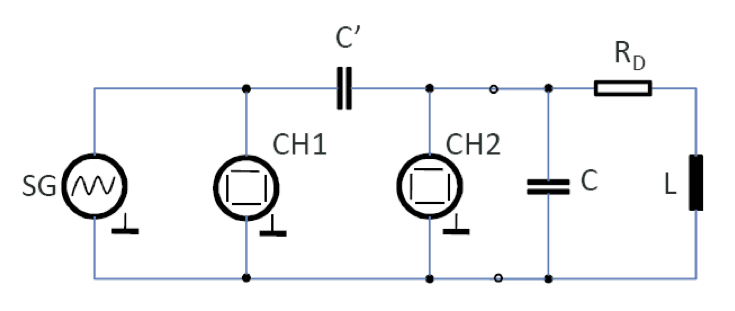
\includegraphics[scale=0.6]{./figure/schwingkreis_aufbau.png}
	\caption{Aufbau der Schaltung des getriebenen Schwingkreises}
	\label{fig:schwingkreis_aufbau}
\end{figure}

Für diesen Versuch bleibt die Schaltung die gleiche. Jetzt erzeugt der Signalgenerator jedoch eine Sinuswelle, eben die antreibende Spannung.\\
Es wird eine Resonanzkurve jeweils für den Fall mit und ohne dem Widerstand $R_D$ gemessen (einzelne Messpunkte von $\omega$ und der davon abhängigen Amplitude).\\
$\omega_{max}$ kann berechnet werden und wird durch die Resonanzkurve genauer bestimmt. Durch Vergleich der Spannungsverläufe an beiden Messpunkten unterhalb und oberhalb dieser Frequenz soll die Phasenverschiebung überprüft werden.\\
Wie in PS1 kann aus der Halbwertsbreite der Resonanzkurve (bei $1/\sqrt{2}$ der MaximalAmplitude) wieder die Dämpfung, Eigenfrequenz und der der Gütefaktor berechnet werden und mit den Ergebnissen aus der ersten Aufgabe verglichen werden.


\subsection{Gekoppelte Schwingkreise}

Für diesen Versuch muss die Schaltung umgebaut werden:\\
Die Bauteile für den Schwingkreis aus den anderen beiden Aufgaben sind doppelt vorhanden und werden wie in Abb.\ref{fig:kopplung_aufbau} geschaltet. Dazu kommt der Kopplungskondensator $C_K$.\\
An den beiden Kanälen des Oszilloskops wird nun der Spannungsverlauf an jeweils einem der beiden Schwingkreise dargestellt, Der Signalgenerator und der Einkopplungs-Kondensator bilden gemeinsam den Treiber.\\

Die gleich- und die gegensinnige Schwingung können hier nicht durch die Anregung erzeugt werden. Als erstes wird daher (wieder mittels Rechteckswelle) eine frei abklingende Schwingung des Systems erzeugt. Am Oszilloskop kann die Schwebungsperiode sowie die Periode der Schwingung der Oszillatoren selbst wieder mittels Cursor gemessen werden.\\
Daraus werden die Kreisfrequenzen $\omega_S$ und $\omega_m$ berechnet und aus diesen die Eigenfrequenzen $\omega_{gl}$ und $\omega_{geg}$.\\
Diese können nun auch direkt gemessen werden, indem das System mit einer Sinuswelle angeregt wird, in der Nähe der beiden berechneten Frequenzwerte, und der Punkt der Resonanz gesucht wird.\\
Wie in PS1, wird nun wieder der Kopplungsgrad auf 2 verschiedene Arten berechnet und verglichen.


\end{multicols}
\begin{figure}[H]
	\centering
	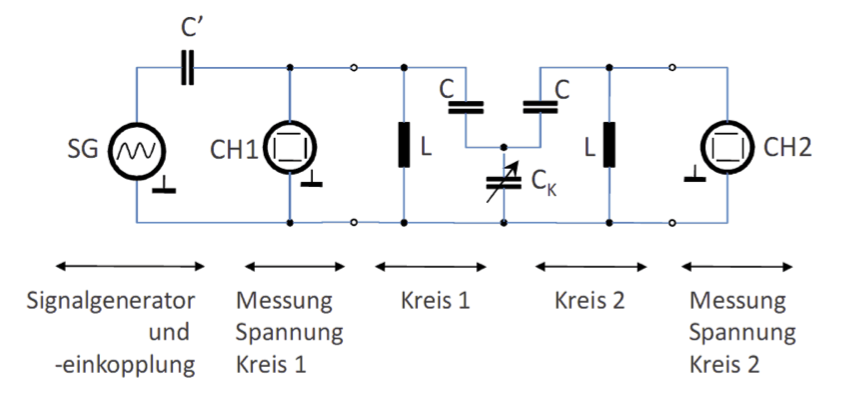
\includegraphics[scale=1.1]{./figure/kopplung_aufbau.png}
	\caption{Aufbau der Schaltung für die Bestimmung der Kopplungskonstante}
	\label{fig:kopplung_aufbau}
\end{figure}
\begin{multicols}{2}


\pagebreak
%%%%%%%%%%%%%%%%%%%%%%%%%%%%%%%%%%%%%%%%%%%%%%%%%%%%%%%%%%%%%%%%%%%%%%%
\section{Resultate}
\subsection{freischwingend}



\end{multicols}
\begin{figure}[H]
	\centering
	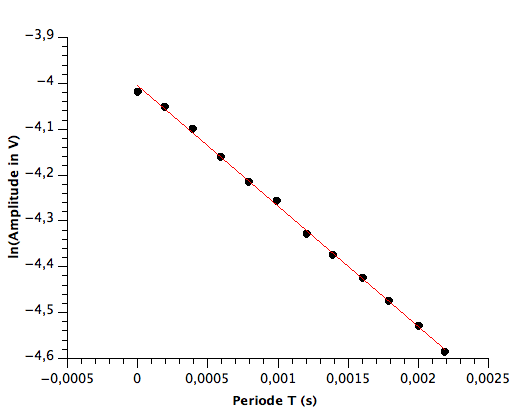
\includegraphics[scale=0.7]{./figure/Schwingkreis_ohne-daempfung.png}
	\caption{freie ungedämpfte Schwingung - ln(A) gegen die Zeit}
	\label{fig:kopplung_aufbau}
\end{figure}
\begin{multicols}{2}



\noindent \textbf{Schwingkreis ohne Dämpfung:}\\

\noindent Es wurde der Kondensator $C_2$ verwendet.\\

\noindent $L=(1.00 \pm 0.03)mH$\\
$T_{Durchschnitt}% = 2.19 / 12 
= (0.183 \pm 0.01)ms$\\
$\omega_{0d} = (34300 \pm 1900)s^{-1}$\\
$R_L = R = (0.525 \pm 0.017)\Omega$

$$\delta_{ungedaempft} = (262.7 \pm 2.9)s^{-1}$$
$$C = (8.50 \pm 0.98)\mu F$$
$$\omega_{0} = (34300\pm 1900)s^{-1}$$

% sqrt((34428.4)^2 + (262.7)^2)


\end{multicols}
\begin{figure}[H]
	\centering
	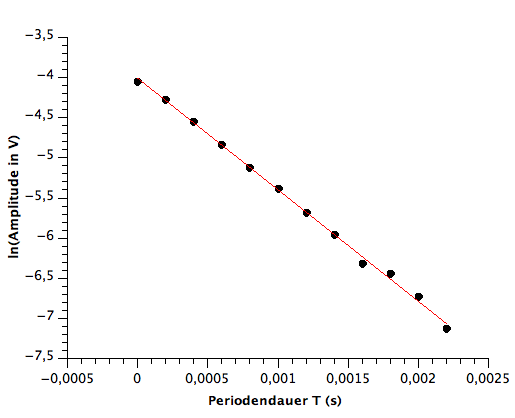
\includegraphics[scale=0.7]{./figure/Schwingkreis_mit2-2ohm-daempfung.png}
	\caption{gedaempft: R = 2.2$\Omega$ - ln(A) gegen die Zeit}
	\label{fig:kopplung_aufbau}
\end{figure}
\begin{multicols}{2}


\noindent \textbf{Schwingkreis mit Dämpfung}\\

\noindent $R_D = (2.20\pm 0.22)\Omega$\\
$L=(1.00 \pm 0.03)mH$\\
$T_{Durchschnitt}% = 2.2 / 12 
= (0.183  \pm 0.01) ms$\\
$\omega_{0d} = (34300 \pm 1900)s^{-1}$\\
$R_L = R-R_D = (0.58 \pm 0.24)\Omega$ 
$$\delta_{gedaempft} = (1390 \pm 21)s^{-1}$$
$$C = (8.50 \pm 0.98)\mu F$$
$$\omega_{0} = 34328 \pm 1900)s^{-1}$$
% sqrt((34278.2)^2 + (1390)^2)


\noindent \textbf{aperiodischer Grenzfall:}
$$R_{apGrenz-gemessen} = (57\pm 3)\Omega$$
$$R_{apGrenz-berechnet}=(68.6 \pm 4.4)\Omega$$

\subsection{Doppel-Schwingkreis}
$$K = 2*2341*35903 /((2341)^2+(35903.9)^2)$$

\pagebreak
%%%%%%%%%%%%%%%%%%%%%%%%%%%%%%%%%%%%%%%%%%%%%%%%%%%%%%%%%%%%%%%%%%%%%%%
\section{Diskussion}

%R_L: der R_D bringt a riesenunsicherheit hinein (etwa faktor 3), ansonsten passts

\subsection{Schwingkreis ohne Dämpfung}



\section{Quellen}
$[1]$ Anleitung, \url{http://www.univie.ac.at/anfpra/neu1/ps/ps2/PS2.pdf}\\
$[2]$ Rohdaten, \url{htts://github.com/blackandcold/Protocols-SS2014-P2/tree/master/PS_2/data}\\

\end{multicols}
\end{document}